\documentclass[11pt,a4paper]{article}

\usepackage[margin=1in]{geometry}
\usepackage{graphicx}
\usepackage{booktabs}
\usepackage{hyperref}
\usepackage{enumitem}
\usepackage{float}
\usepackage{caption}
\usepackage{xcolor}
\usepackage{titlesec}
\usepackage{fancyhdr}

\hypersetup{
  colorlinks=true,
  linkcolor=black,
  urlcolor=blue
}

\pagestyle{fancy}
\fancyhf{}
\fancyhead[L]{Gabilla --- ML Web App Documentation}
\fancyhead[R]{MCAIPAT}
\fancyfoot[C]{\thepage}

\title{Technical Documentation:\\Developing a Web Application Prototype\\with Integrated Supervised Machine Learning Model}
\author{Cyrus Gabilla}
\date{\today}

\begin{document}
\maketitle

\begin{abstract}
This report documents the development of a local Flask web application that integrates a previously trained Gaussian Naive Bayes pipeline for predicting whether a Portuguese secondary-school student is at risk of failing (\texttt{AtRisk} when final grade \(G3 < 10\)). The application accepts student background and school-related inputs without using period or final grades as features, loads a locally saved \texttt{joblib} model, and returns a prediction with probabilities and post-hoc insights. The system runs fully offline.
\end{abstract}

\tableofcontents
\newpage

%% ============================================================
\section{Introduction}
%% ============================================================

This laboratory builds on a supervised machine learning project that predicted student at-risk status from the UCI Student Performance (Portuguese) dataset. The goal of this activity is to turn that trained model into a practical local web prototype: a user enters student attributes in a browser form, the backend loads the exported model, and the interface displays the predicted outcome.

The application title presented to users is ``Will this student pass Portuguese?'' The assignment activity title is \emph{Developing a Web App Prototype with Integrated SML Prediction Model}.

%% ============================================================
\section{Overview of the Previous Machine Learning Project}
%% ============================================================

\begin{itemize}[leftmargin=*]
  \item \textbf{Dataset:} UCI Student Performance --- Portuguese language course (\texttt{student\_performance.csv} / \texttt{student-por.csv}).
  \item \textbf{Problem type:} Binary classification.
  \item \textbf{Target:} \texttt{AtRisk} \(= 1\) if \(G3 < 10\), else \(0\) (Cortez \& Silva, 2008 binary pass/fail definition).
  \item \textbf{Features:} 30 attributes after dropping \texttt{G1}, \texttt{G2}, and \texttt{G3} (early-warning setup).
  \item \textbf{Algorithms compared:} Support Vector Machine, Gaussian Naive Bayes, and Gradient Boosting.
  \item \textbf{Selected model:} Gaussian Naive Bayes (best F1 / recall for the rare at-risk class).
  \item \textbf{Preprocessing:} \texttt{StandardScaler} for numeric columns and \texttt{OneHotEncoder} for categorical columns inside a scikit-learn \texttt{Pipeline}.
\end{itemize}

Naive Bayes was selected for integration because, although Support Vector Machine had slightly higher accuracy, Naive Bayes better identified at-risk students (higher F1 and recall). For an early-warning tool, catching students who may need support matters more than overall accuracy alone.

%% ============================================================
\section{Model Export and Preparation}
%% ============================================================

The fitted preprocessing-and-model pipeline was exported with Joblib so the web app can apply the same encoding and scaling used during training.

\begin{verbatim}
import joblib
from google.colab import files

best_model = trained["Naive Bayes"]
joblib.dump(best_model, "trained_model.joblib")
print("Model successfully saved!")
files.download("trained_model.joblib")
\end{verbatim}

Model persistence is necessary because the web application must generate predictions offline without reconnecting to Google Colab or a cloud prediction API.

\begin{figure}[H]
  \centering
  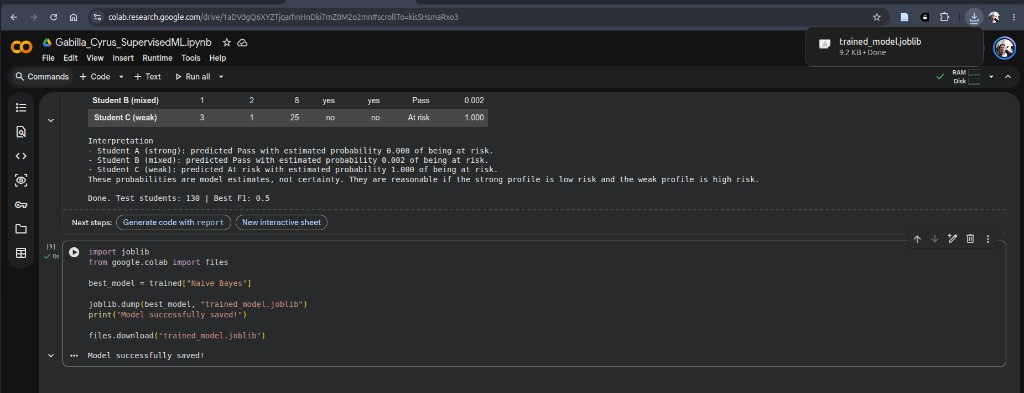
\includegraphics[width=0.95\textwidth]{../screenshots/activity02/01-colab-export-and-download.png}
  \caption{Exporting and downloading the Naive Bayes pipeline (\texttt{trained\_model.joblib}) from Google Colab.}
  \label{fig:colab-export}
\end{figure}

\begin{figure}[H]
  \centering
  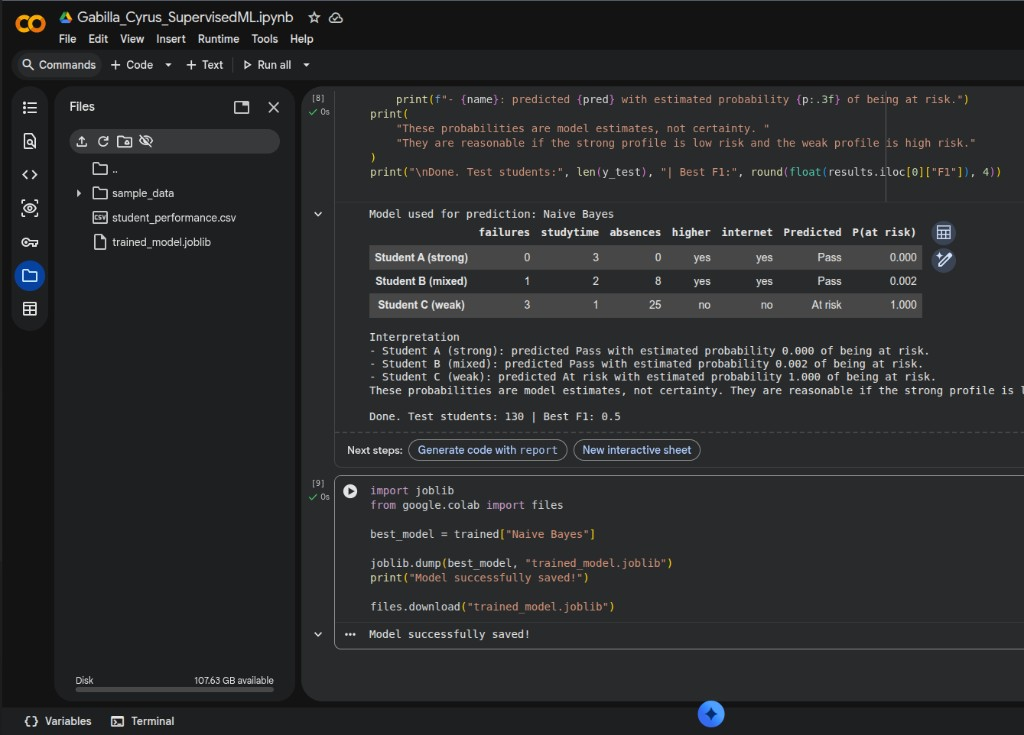
\includegraphics[width=0.95\textwidth]{../screenshots/activity02/02-colab-files-trained-model.png}
  \caption{Google Colab Files panel showing the generated \texttt{trained\_model.joblib} beside the dataset file.}
  \label{fig:colab-files}
\end{figure}

The figure confirms that the Joblib artifact was written inside the Colab runtime before download. The same file was later copied into the local web project \texttt{model/} directory for offline inference.

%% ============================================================
\section{Development Environment Setup}
%% ============================================================

\begin{itemize}[leftmargin=*]
  \item \textbf{Language / framework:} Python 3.12, Flask
  \item \textbf{ML stack:} scikit-learn 1.6.1, joblib, pandas, PyYAML
  \item \textbf{Frontend:} HTML, CSS, JavaScript
  \item \textbf{Editor:} local IDE / code editor
  \item \textbf{Install:} \texttt{python3 -m venv .venv \&\& pip install -r requirements.txt}
\end{itemize}

\begin{figure}[H]
  \centering
  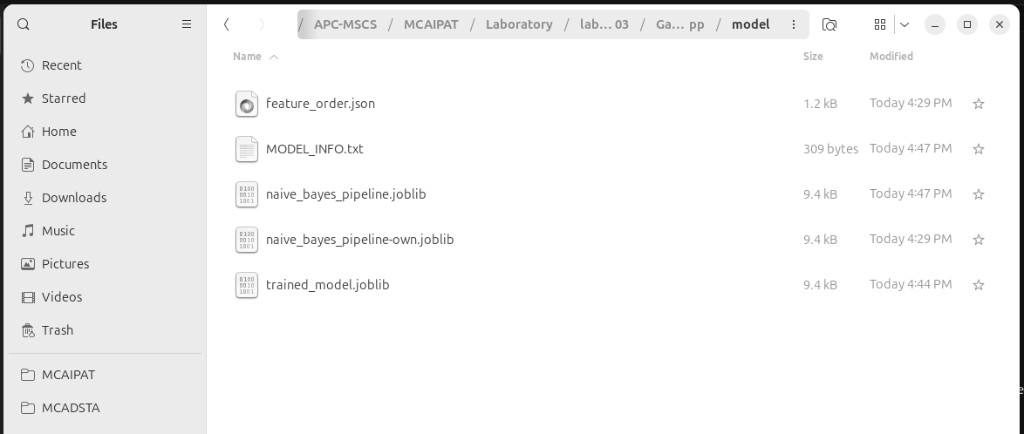
\includegraphics[width=0.92\textwidth]{../screenshots/activity03/01-local-model-folder.png}
  \caption{Local project \texttt{model/} directory containing the exported Joblib pipeline (\texttt{trained\_model.joblib} / \texttt{naive\_bayes\_pipeline.joblib}) used by the Flask app.}
  \label{fig:local-model}
\end{figure}

\begin{figure}[H]
  \centering
  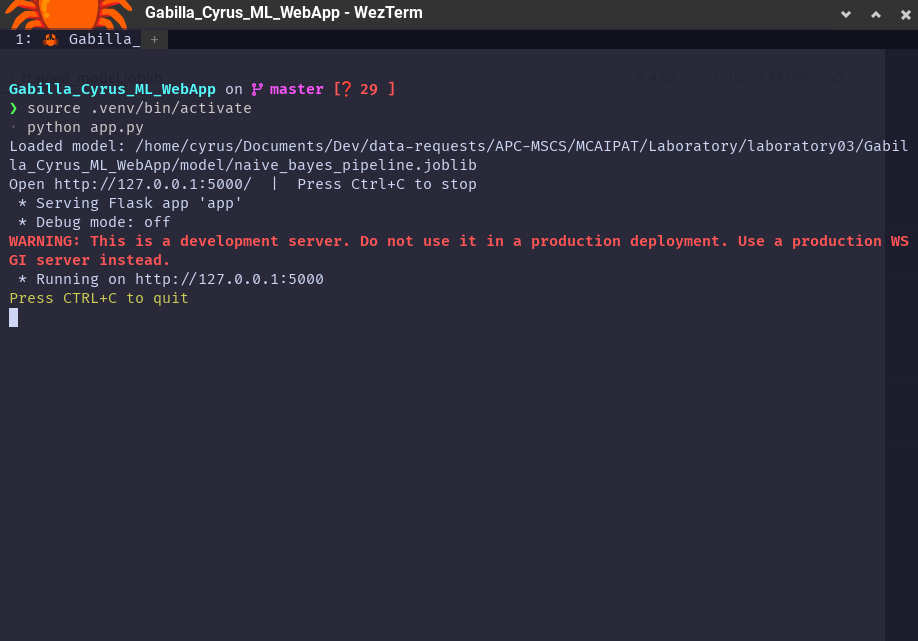
\includegraphics[width=0.95\textwidth]{../screenshots/activity03/02-python-app-running.png}
  \caption{Local development server started with \texttt{source .venv/bin/activate} and \texttt{python app.py}, loading the Naive Bayes pipeline and serving \texttt{http://127.0.0.1:5000/}.}
  \label{fig:app-running}
\end{figure}

%% ============================================================
\section{Web Application Interface Development}
%% ============================================================

The interface includes:
\begin{enumerate}
  \item Application title and short description
  \item About / how-to-use information
  \item Grouped input form for all 30 training features
  \item Predict and Clear actions
  \item Result panel with probabilities and post-prediction insights
  \item Optional ``Surprise me'' random profile filler (fills inputs only; prediction still uses the model)
\end{enumerate}

Fields are left empty by default. Clear resets to blank values. Missing inputs show validation messages asking the user to complete the form.

\begin{figure}[H]
  \centering
  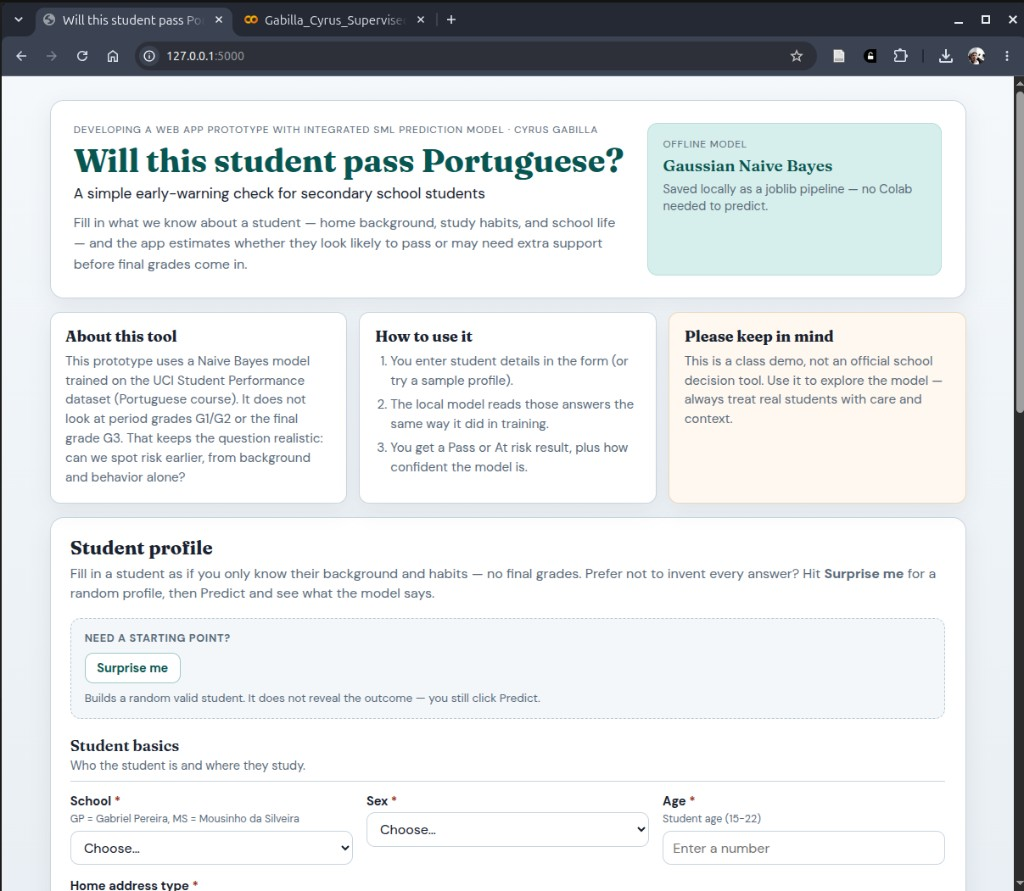
\includegraphics[width=0.95\textwidth]{../screenshots/activity04/01-homepage-top.png}
  \caption{Web application homepage: title, about/how-to panels, offline model note, and the start of the empty student form.}
  \label{fig:ui-top}
\end{figure}

\begin{figure}[H]
  \centering
  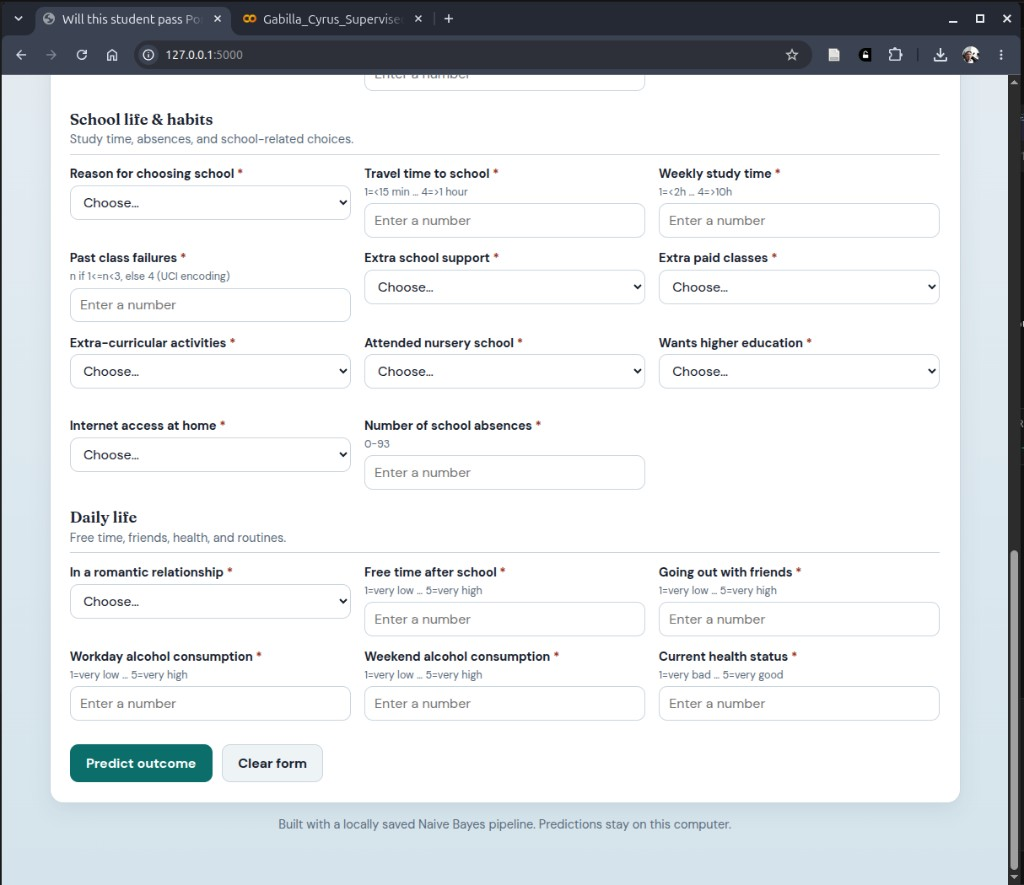
\includegraphics[width=0.95\textwidth]{../screenshots/activity04/02-homepage-form-bottom.png}
  \caption{Remaining grouped form sections (school life and daily life) with empty inputs, plus Predict and Clear actions.}
  \label{fig:ui-bottom}
\end{figure}

The interface keeps all required features visible but blank by default so users must enter values (or use Surprise me) before prediction.

%% ============================================================
\section{Machine Learning Model Integration}
%% ============================================================

The exported model was placed under \texttt{model/} (as \texttt{trained\_model.joblib} / \texttt{naive\_bayes\_pipeline.joblib}). Flask loads the pipeline at startup with Joblib. On \texttt{POST /predict}, the backend validates inputs, builds a one-row DataFrame in training feature order, calls \texttt{predict} / \texttt{predict\_proba}, and renders the result.

\begin{verbatim}
PIPELINE = joblib.load(MODEL_PATH)
...
pred = PIPELINE.predict(frame)[0]
proba = PIPELINE.predict_proba(frame)[0]
\end{verbatim}

This keeps preprocessing and classification identical to training and avoids hard-coded outcomes.

Figure~\ref{fig:local-model} already shows the saved model inside the project directory. The Flask backend loads this file at startup and uses it for every prediction request.

\noindent\textit{Pending screenshots: code editor view of model loading (optional); prediction evidence appears in the testing section.}

%% ============================================================
\section{Application Testing and Results}
%% ============================================================

\subsection*{Test 1 --- Successful prediction (Likely to pass)}
A completed student profile was submitted through the web form. The local Naive Bayes pipeline returned class \texttt{Pass} (\texttt{AtRisk = 0}) with a very high estimated chance of passing. The result panel also listed post-prediction notes (for example, wanting higher education and solid study habits).

\begin{figure}[H]
  \centering
  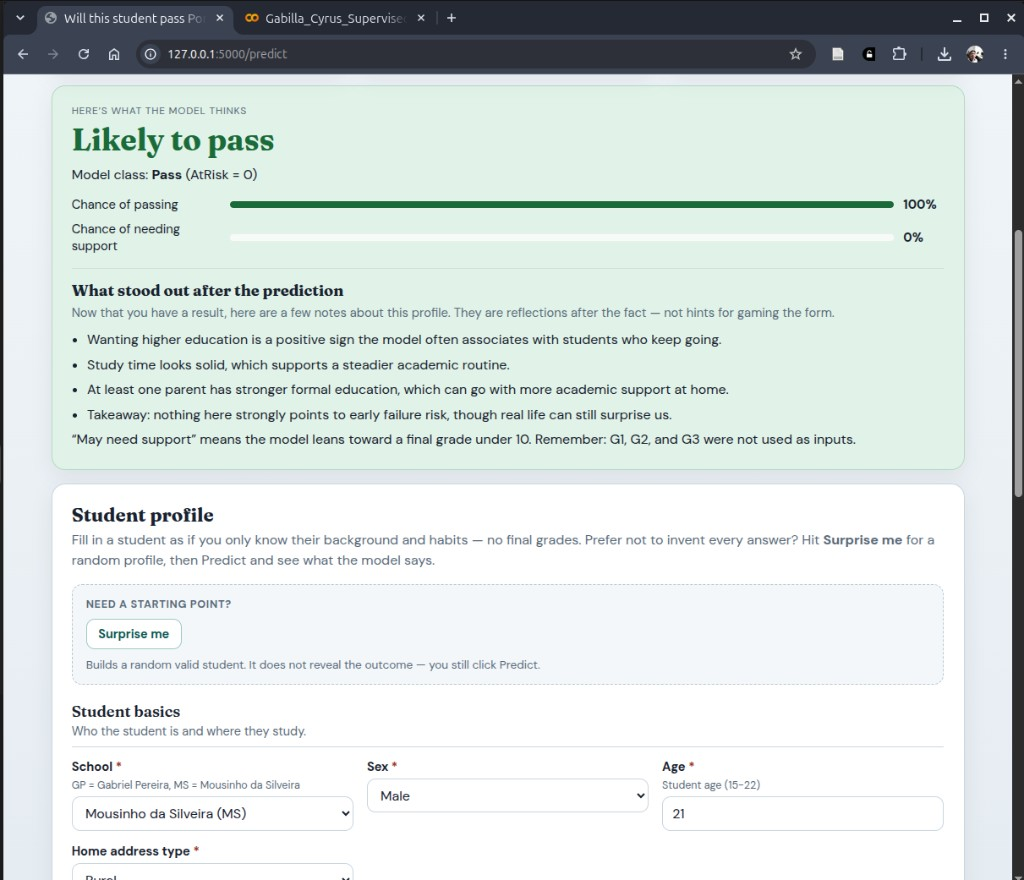
\includegraphics[width=0.95\textwidth]{../screenshots/activity06/01-predict-pass.png}
  \caption{Successful prediction test 1: model output ``Likely to pass'' / Pass (\texttt{AtRisk = 0}) with probability bars and insights.}
  \label{fig:test-pass}
\end{figure}

\subsection*{Test 2 --- Successful prediction (May need support)}
A different profile was submitted. The same offline pipeline returned class \texttt{At risk} (\texttt{AtRisk = 1}) with a high estimated chance of needing support. Insights highlighted concerning answers such as high absences and elevated social/alcohol indicators.

\begin{figure}[H]
  \centering
  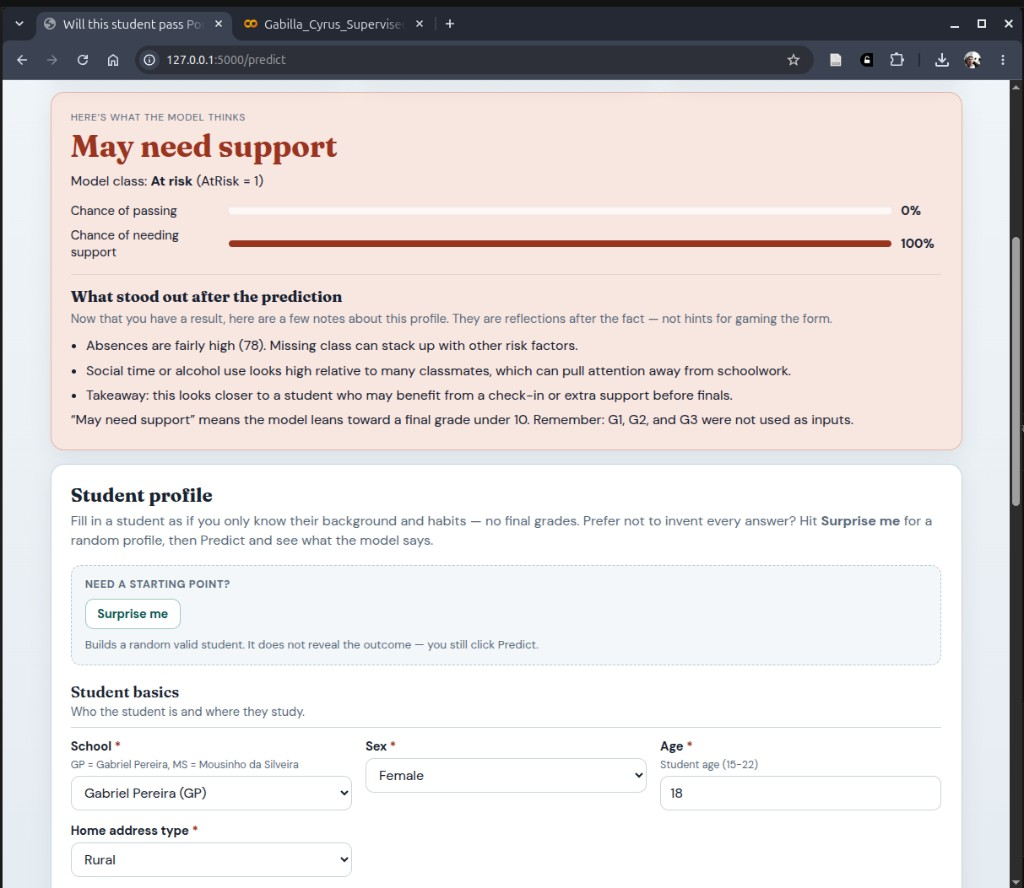
\includegraphics[width=0.95\textwidth]{../screenshots/activity06/02-predict-at-risk.png}
  \caption{Successful prediction test 2: model output ``May need support'' / At risk (\texttt{AtRisk = 1}) with probability bars and insights.}
  \label{fig:test-risk}
\end{figure}

\subsection*{Test 3 --- Successful prediction (shared probability mass)}
A third profile was submitted. The model again predicted Pass, but with a more balanced probability split (about 79\% chance of passing and 21\% chance of needing support). This shows that \texttt{predict\_proba} can return non-extreme confidence values, not only 0\%/100\% outcomes.

\begin{figure}[H]
  \centering
  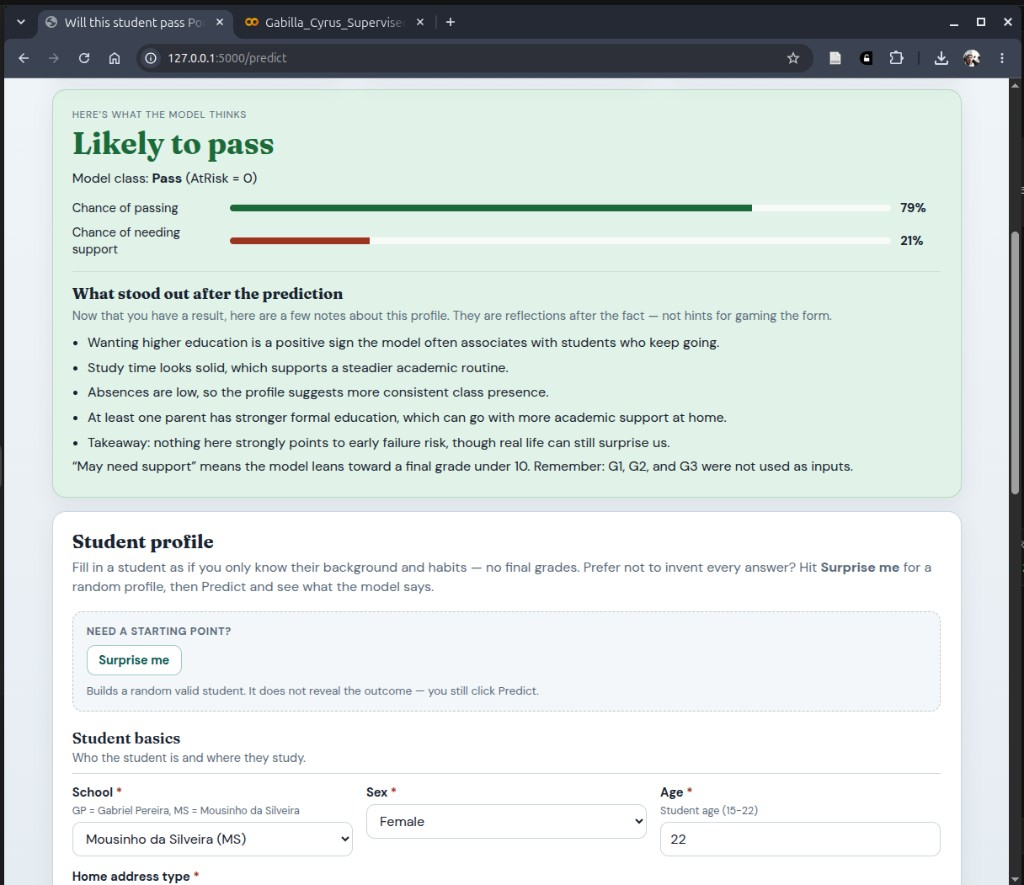
\includegraphics[width=0.95\textwidth]{../screenshots/activity06/03-predict-pass-mixed-proba.png}
  \caption{Successful prediction test 3: Pass result with both probability bars populated (approximately 79\% / 21\%).}
  \label{fig:test-mixed}
\end{figure}

\subsection*{Test 4 --- Validation / error handling}
After clearing the form, Predict was clicked with empty required fields. Client-side validation blocked submission and displayed a message that some fields are still empty, listing missing inputs such as School, Sex, and Age. This confirms the application does not invent a prediction when data is incomplete.

\begin{figure}[H]
  \centering
  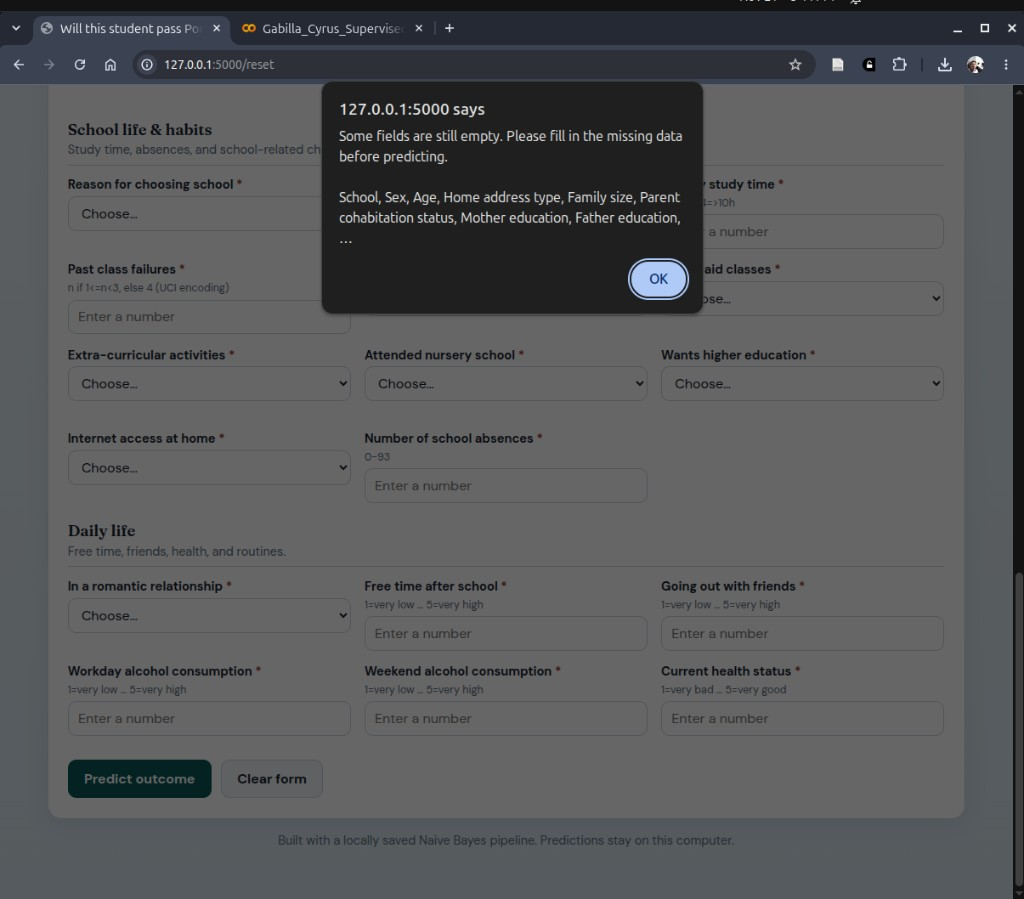
\includegraphics[width=0.95\textwidth]{../screenshots/activity06/04-validation-missing-fields.png}
  \caption{Validation test: empty form triggers a missing-data warning instead of a prediction.}
  \label{fig:test-validation}
\end{figure}

%% ============================================================
\section{Offline Functionality Verification}
%% ============================================================

Predictions are produced by the local \texttt{.joblib} file inside the project. The running app does not call Google Colab or an external prediction API. Evidence includes the local model directory (Figure~\ref{fig:local-model}), the Flask process loading that file (Figure~\ref{fig:app-running}), and live browser predictions at \texttt{http://127.0.0.1:5000/} (Figures~\ref{fig:test-pass},~\ref{fig:test-risk}, and~\ref{fig:test-mixed}).

%% ============================================================
\section{AI-Assisted Coding Disclosure}
%% ============================================================

AI-assisted coding was used during development. In particular, \textbf{Gemini} was consulted for ideas on web app structure, Flask integration, clearer UI wording, and documentation drafts.

All AI-generated suggestions were reviewed by the student author, adapted to the actual Laboratory feature set and exported Naive Bayes pipeline, and verified through local testing (\texttt{python app.py}, form validation for missing inputs, and live predictions from the saved \texttt{joblib} model). No prediction results in this application are hard-coded; outputs come from the locally loaded model.

This disclosure is provided in narrative form. Separate AI chat screenshots are not included with this report.

%% ============================================================
\section{Challenges and Observations}
%% ============================================================

\begin{itemize}[leftmargin=*]
  \item Saving the full Pipeline (not only the classifier) was essential so OneHot encoding and scaling stay consistent at inference time.
  \item YAML \texttt{yes}/\texttt{no} values can be parsed as booleans; they were quoted as strings for form validation.
  \item The Colab export used scikit-learn 1.6.1, so the local environment was aligned to avoid load warnings.
  \item UI defaults were removed so Clear truly empties the form and missing-field validation is visible.
\end{itemize}

%% ============================================================
\section{Conclusion}
%% ============================================================

This project demonstrates the path from a notebook-trained supervised model to a usable local web application. A user can enter student attributes, the Flask backend loads the exported Naive Bayes pipeline, and the interface presents a Pass / at-risk style outcome with probabilities. The prototype satisfies the laboratory requirement of offline, model-driven prediction without depending on Colab at runtime.

%% ============================================================
\section{References}
%% ============================================================

\begin{enumerate}[leftmargin=*]
  \item Cortez, P., \& Silva, A. (2008). \emph{Using Data Mining to Predict Secondary School Student Performance.} University of Minho.
  \item UCI Machine Learning Repository. Student Performance Data Set. \url{https://archive.ics.uci.edu/dataset/320/student+performance}
  \item Flask documentation. \url{https://flask.palletsprojects.com/}
  \item scikit-learn documentation (Pipeline, GaussianNB, joblib model persistence).
  \item Laboratory handout: \emph{Developing a Web App Prototype with Integrated SML Prediction Model.}
\end{enumerate}

\end{document}
